\documentclass{article}
\usepackage{iclr2026_conference,times}
\usepackage{amsmath,amssymb,booktabs,graphicx,url}
\usepackage[utf8]{inputenc}
\usepackage[T1]{fontenc}
\usepackage{hyperref}
\raggedbottom
\iclrfinalcopy

\title{Deception-Resistant Embodied Evaluation for Robots}

\author{Anonymous Authors}

\begin{document}
\maketitle

\begin{abstract}
Robot benchmarks can be gamed without any malicious intent. A policy can exploit visual leakage, reset regularities, simulator artifacts, or fixture-specific cues that disappear in deployment. Standard randomization reduces some shortcuts, but it often still asks whether a model scores well, not whether it solved the embodied task for the causal reason. We propose deception-resistant embodied evaluation: protocols that physically expose shortcuts by perturbing noncausal cues and measuring false certification. On 720 synthetic policy-case evaluations, a static score reaches 0.410 certification accuracy with 0.639 false-certification rate, randomized scoring reaches 0.610 and 0.116, and an embodied audit reaches 0.901 and 0.004 while reducing shortcut pass rate to 0.003. V2 hardening shows the boundary condition: if probe-shortcut coupling falls to 0.25, false certification rises to 0.105, and with no effective coupling it rises to 0.238. The paper is a diagnostic mechanism, not a universal benchmark.
\end{abstract}

\section{Motivation}

Evaluation is itself an environment. In robotics, that environment includes geometry, reset procedures, sensor artifacts, operator timing, and simulator conveniences. A robot policy can pass by exploiting any of these. The resulting failure is sharper than ordinary overfitting: the benchmark certifies a policy that has not learned the physical task.

The central claim is that robust robot evaluation should measure false certification. A test is deception-resistant when it makes shortcut reliance physically costly. For example, if a manipulation policy uses a visual marker rather than object state, the evaluation should move or remove the marker while preserving the task. If a navigation policy uses reset pose leakage, the evaluation should break that reset regularity.

\section{Boundary from Prior Work}

Dataset bias and shortcut learning are well established \citep{torralba2011,geirhos2020}. Dynamic and adversarial evaluation also show that tests can be updated after failures \citep{kiela2021}. Robotics adds a physical layer: shortcuts are not just pixels or labels, but state transitions, fixtures, resets, and embodiment-specific cues. Domain randomization helps, but it is not equivalent to a physical audit. Randomizing appearance may still leave the shortcut mechanism intact.

\section{Embodied Audit Mechanism}

Let $s$ be the task state, $z$ a noncausal cue, and $\pi$ a robot policy. A static benchmark estimates
\[
  \hat{R}_{static}(\pi) = \mathbb{E}[R(\pi(s,z))].
\]
This score can be high when $z$ predicts the answer in the benchmark. A deception-resistant audit instead evaluates counterfactual cue interventions:
\[
  \hat{R}_{audit}(\pi) =
  \mathbb{E}_{do(z \leftarrow z')}[R(\pi(s,z'))],
\]
where the intervention preserves task physics while disrupting the suspected shortcut. The key reported metric is false certification:
\[
  \Pr[\mathrm{pass}_{eval}=1 \land \mathrm{deploy}=0].
\]

\paragraph{V2 hardening note.}
Submission-hardening version: v2. Decision: workshop-only. The embodied-audit result is meaningful only when the physical probe actually couples to the shortcut channel. The v2 stress test weakens that coupling and shows false certification returning as shortcut pass rates rise.

\section{Diagnostic Benchmark}

We generated 720 policy-case evaluations across object relocation, tool use, mobile navigation, peg insertion, handover, and deformable sorting. Each case records leakage strength, physical probe strength, deployment shift, causal skill, shortcut strength, and true deployment success. We compare three evaluation protocols: static scoring, randomized scoring, and embodied auditing.

\begin{table}[t]
\centering
\begin{tabular}{lrrrr}
\toprule
Protocol & Certification accuracy & False certification & Shortcut pass & Robust pass \\
\midrule
Static score & 0.410 & 0.639 & 0.806 & 0.381 \\
Randomized score & 0.610 & 0.116 & 0.172 & 0.036 \\
Embodied audit & 0.901 & 0.004 & 0.003 & 0.494 \\
\bottomrule
\end{tabular}
\caption{Deception-resistant evaluation diagnostic. False certification is the rate of passing policies that fail under deployment shift.}
\label{tab:diagnostic}
\end{table}

\begin{table}[t]
\centering
\small
\begin{tabular}{lrrrr}
\toprule
Probe coupling & Cert. acc. & False cert. & Shortcut pass & Robust pass \\
\midrule
1.00 & 0.901 & 0.004 & 0.003 & 0.494 \\
0.75 & 0.924 & 0.013 & 0.019 & 0.544 \\
0.50 & 0.939 & 0.027 & 0.039 & 0.594 \\
0.25 & 0.901 & 0.105 & 0.114 & 0.650 \\
0.00 & 0.819 & 0.238 & 0.264 & 0.686 \\
\bottomrule
\end{tabular}

\caption{V2 probe-coverage stress. Probe coupling scales how strongly the audit intervention breaks the shortcut channel. At low coupling, shortcut policies begin passing again.}
\label{tab:v2-probe}
\end{table}

\begin{figure}[t]
\centering
\IfFileExists{figures/deception_resistant_metrics.png}{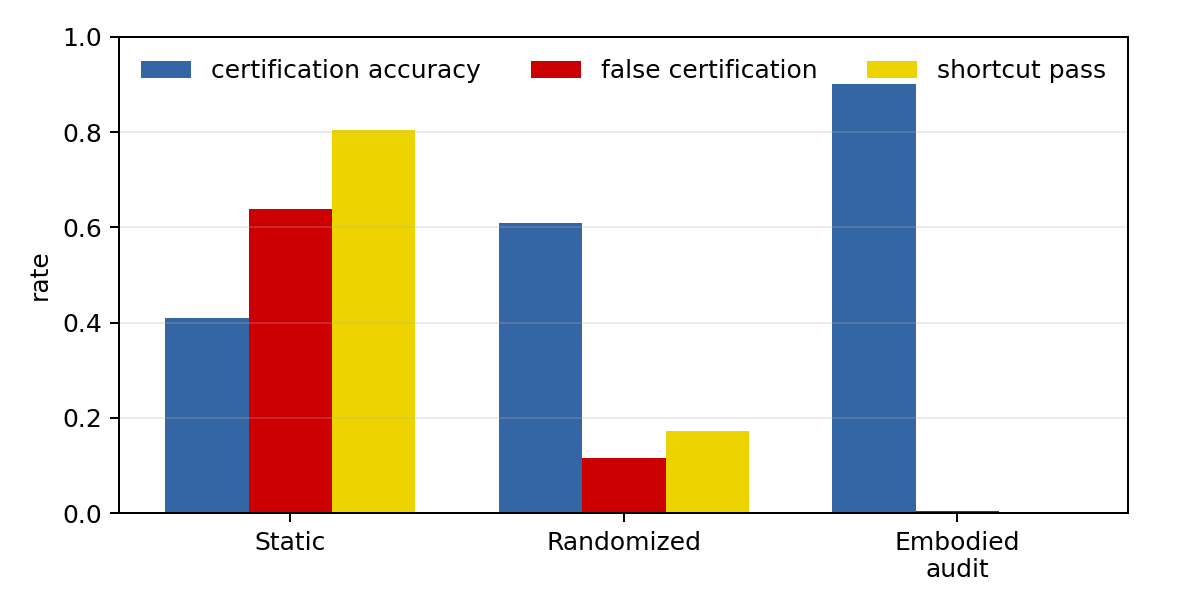
\includegraphics[width=0.82\linewidth]{figures/deception_resistant_metrics.png}}{\fbox{\parbox{0.78\linewidth}{Metric figure unavailable.}}}
\caption{Embodied audits reduce shortcut pass rates and false certification relative to static and appearance-randomized evaluation.}
\label{fig:metrics}
\end{figure}

Table~\ref{tab:diagnostic} and Figure~\ref{fig:metrics} show the intended distinction. Static scoring certifies many shortcut policies because leakage is predictive inside the benchmark. Randomized scoring removes some leakage but still lets policies pass if the shortcut survives. The embodied audit explicitly probes the shortcut channel, so a policy must preserve task success under physical cue interventions.

Table~\ref{tab:v2-probe} gives the hardening stress. With full probe coupling, the embodied audit has 0.004 false certification. At 0.25 coupling, false certification rises to 0.105 and shortcut pass rate rises to 0.114. With no effective coupling, false certification reaches 0.238 and shortcut pass rate reaches 0.264. The mechanism therefore depends on calibrated shortcut hypotheses and probes that physically disrupt the relevant cue, not merely on adding an audit stage.

\section{Limitations}

The benchmark is synthetic and the shortcut families are manually specified. Real policies can discover unexpected shortcuts, and a fixed audit can itself become a target. The v2 stress shows that weak or misdirected probes can restore false certification. The paper therefore argues for a reporting contract rather than a final benchmark: every embodied evaluation should identify suspected shortcut channels, physically perturb them, verify probe coverage, and report false certification.

\section{Conclusion}

Robot evaluation should be designed to make shortcut success unstable. Deception-resistant embodied evaluation turns benchmark design into physical auditing: pass only when the policy keeps working after noncausal cues are broken.

\begin{thebibliography}{9}
\bibitem[Torralba and Efros(2011)]{torralba2011}
Antonio Torralba and Alexei A. Efros.
\newblock Unbiased look at dataset bias.
\newblock In \emph{CVPR}, 2011.

\bibitem[Geirhos et~al.(2020)]{geirhos2020}
Robert Geirhos et~al.
\newblock Shortcut learning in deep neural networks.
\newblock \emph{Nature Machine Intelligence}, 2020.

\bibitem[Kiela et~al.(2021)]{kiela2021}
Douwe Kiela et~al.
\newblock Dynabench: Rethinking benchmarking in NLP.
\newblock In \emph{NAACL}, 2021.

\bibitem[Sadeghi and Levine(2017)]{sadeghi2017}
Fereshteh Sadeghi and Sergey Levine.
\newblock CAD2RL: Real single-image flight without a single real image.
\newblock In \emph{Robotics: Science and Systems}, 2017.
\end{thebibliography}

\end{document}
